\documentclass{article}
\usepackage[margin=1in]{geometry}
\usepackage[linesnumbered,ruled,vlined]{algorithm2e}
\usepackage{amsfonts}
\usepackage{amsmath}
\usepackage{amssymb}
\usepackage{amsthm}
\usepackage{enumitem}
\usepackage{fancyhdr}
\usepackage{hyperref}
\usepackage{minted}
\usepackage{multicol}
\usepackage{pdfpages}
\usepackage{standalone}
\usepackage[many]{tcolorbox}
\usepackage{tikz-cd}
\usepackage{transparent}
\usepackage{xcolor}
% \tcbuselibrary{minted}

\author{Nathan Solomon}

\newcommand{\fig}[1]{
    \begin{center}
        \includegraphics[width=\textwidth]{#1}
    \end{center}
}

% Math commands
\renewcommand{\d}{\mathrm{d}}
\DeclareMathOperator{\id}{id}
\DeclareMathOperator{\im}{im}
\DeclareMathOperator{\proj}{proj}
\DeclareMathOperator{\Span}{span}
\DeclareMathOperator{\Tr}{Tr}
\DeclareMathOperator{\tr}{tr}
\DeclareMathOperator{\ad}{ad}
\DeclareMathOperator{\ord}{ord}
%%%%%%%%%%%%%%% \DeclareMathOperator{\sgn}{sgn}
\DeclareMathOperator{\Aut}{Aut}
\DeclareMathOperator{\Inn}{Inn}
\DeclareMathOperator{\Out}{Out}
\DeclareMathOperator{\stab}{stab}

\newcommand{\N}{\ensuremath{\mathbb{N}}}
\newcommand{\Z}{\ensuremath{\mathbb{Z}}}
\newcommand{\Q}{\ensuremath{\mathbb{Q}}}
\newcommand{\R}{\ensuremath{\mathbb{R}}}
\newcommand{\C}{\ensuremath{\mathbb{C}}}
\renewcommand{\H}{\ensuremath{\mathbb{H}}}
\newcommand{\F}{\ensuremath{\mathbb{F}}}

\newcommand{\E}{\ensuremath{\mathbb{E}}}
\renewcommand{\P}{\ensuremath{\mathbb{P}}}

\newcommand{\es}{\ensuremath{\varnothing}}
\newcommand{\inv}{\ensuremath{^{-1}}}
\newcommand{\eps}{\ensuremath{\varepsilon}}
\newcommand{\del}{\ensuremath{\partial}}
\renewcommand{\a}{\ensuremath{\alpha}}

\newcommand{\abs}[1]{\ensuremath{\left\lvert #1 \right\rvert}}
\newcommand{\norm}[1]{\ensuremath{\left\lVert #1\right\rVert}}
\newcommand{\mean}[1]{\ensuremath{\left\langle #1 \right\rangle}}
\newcommand{\floor}[1]{\ensuremath{\left\lfloor #1 \right\rfloor}}
\newcommand{\ceil}[1]{\ensuremath{\left\lceil #1 \right\rceil}}
\newcommand{\bra}[1]{\ensuremath{\left\langle #1 \right\rvert}}
\newcommand{\ket}[1]{\ensuremath{\left\lvert #1 \right\rangle}}
\newcommand{\braket}[2]{\ensuremath{\left.\left\langle #1\right\vert #2 \right\rangle}}

\newcommand{\catname}[1]{{\normalfont\textbf{#1}}}

\newcommand{\up}{\ensuremath{\uparrow}}
\newcommand{\down}{\ensuremath{\downarrow}}

% Custom environments
\newtheorem{thm}{Theorem}[section]

\definecolor{probBackgroundColor}{RGB}{250,240,240}
\definecolor{probAccentColor}{RGB}{140,40,0}
\newenvironment{prob}{
    \stepcounter{thm}
    \begin{tcolorbox}[
        boxrule=1pt,
        sharp corners,
        colback=probBackgroundColor,
        colframe=probAccentColor,
        borderline west={4pt}{0pt}{probAccentColor},
        breakable
    ]
    \color{probAccentColor}\textbf{Problem \thethm.} \color{black}
} {
    \end{tcolorbox}
}

\definecolor{exampleBackgroundColor}{RGB}{212,232,246}
\newenvironment{example}{
    \stepcounter{thm}
    \begin{tcolorbox}[
      boxrule=1pt,
      sharp corners,
      colback=exampleBackgroundColor,
      breakable
    ]
    \textbf{Example \thethm.}
} {
    \end{tcolorbox}
}

\definecolor{propBackgroundColor}{RGB}{255,245,220}
\definecolor{propAccentColor}{RGB}{150,100,0}
\newenvironment{prop}{
    \stepcounter{thm}
    \begin{tcolorbox}[
        boxrule=1pt,
        sharp corners,
        colback=propBackgroundColor,
        colframe=propAccentColor,
        breakable
    ]
    \color{propAccentColor}\textbf{Proposition \thethm. }\color{black}
} {
    \end{tcolorbox}
}

\definecolor{thmBackgroundColor}{RGB}{235,225,245}
\definecolor{thmAccentColor}{RGB}{50,0,100}
\renewenvironment{thm}{
    \stepcounter{thm}
    \begin{tcolorbox}[
        boxrule=1pt,
        sharp corners,
        colback=thmBackgroundColor,
        colframe=thmAccentColor,
        breakable
    ]
    \color{thmAccentColor}\textbf{Theorem \thethm. }\color{black}
} {
    \end{tcolorbox}
}

\definecolor{corBackgroundColor}{RGB}{240,250,250}
\definecolor{corAccentColor}{RGB}{50,100,100}
\newenvironment{cor}{
    \stepcounter{thm}
    \begin{tcolorbox}[
        enhanced,
        boxrule=0pt,
        frame hidden,
        sharp corners,
        colback=corBackgroundColor,
        borderline west={4pt}{0pt}{corAccentColor},
        breakable
    ]
    \color{corAccentColor}\textbf{Corollary \thethm. }\color{black}
} {
    \end{tcolorbox}
}

\definecolor{lemBackgroundColor}{RGB}{255,245,235}
\definecolor{lemAccentColor}{RGB}{250,125,0}
\newenvironment{lem}{
    \stepcounter{thm}
    \begin{tcolorbox}[
        enhanced,
        boxrule=0pt,
        frame hidden,
        sharp corners,
        colback=lemBackgroundColor,
        borderline west={4pt}{0pt}{lemAccentColor},
        breakable
    ]
    \color{lemAccentColor}\textbf{Lemma \thethm. }\color{black}
} {
    \end{tcolorbox}
}

\definecolor{proofBackgroundColor}{RGB}{255,255,255}
\definecolor{proofAccentColor}{RGB}{80,80,80}
\renewenvironment{proof}{
    \begin{tcolorbox}[
        enhanced,
        boxrule=1pt,
        sharp corners,
        colback=proofBackgroundColor,
        colframe=proofAccentColor,
        borderline west={4pt}{0pt}{proofAccentColor},
        breakable
    ]
    \color{proofAccentColor}\emph{\textbf{Proof. }}\color{black}
} {
    \qed \end{tcolorbox}
}

\definecolor{noteBackgroundColor}{RGB}{240,250,240}
\definecolor{noteAccentColor}{RGB}{30,130,30}
\newenvironment{note}{
    \begin{tcolorbox}[
        enhanced,
        boxrule=0pt,
        frame hidden,
        sharp corners,
        colback=noteBackgroundColor,
        borderline west={4pt}{0pt}{noteAccentColor},
        breakable
    ]
    \color{noteAccentColor}\textbf{Note. }\color{black}
} {
    \end{tcolorbox}
}


\fancyhf{}
\setlength{\headheight}{24pt}

\date{\today}
\title{Physics 245 Homework \#9}

\begin{document}
\maketitle

\begin{prob}
\end{prob}
\begin{enumerate}[label=(\alph*)]
    \item
        \[ \rho = \frac{1}{2} \left( I + r_x \sigma_x + r_y \sigma_y + r_z \sigma_z \right) = \frac{1}{2} \begin{bmatrix}
            1+r_z & r_x-ir_y \\
            r_x+ir_y & 1-r_z
        \end{bmatrix}. \]
    \item \begin{align*}
            [\sigma_x] &= \tr(\sigma_x \rho) \\
                       &= \tr \left( \frac{1}{2} \begin{bmatrix}
                               0 & 1 \\
                               1 & 0
                       \end{bmatrix} \begin{bmatrix}
                               1+r_z & r_x-ir_y \\
                               r_x+ir_y & 1-r_z
                       \end{bmatrix} \right) \\
                       &= \frac{1}{2} \tr \left( \begin{bmatrix}
                               r_x+ir_y & 1-r_z \\
                               1+r_z & r_x-ir_y
                       \end{bmatrix} \right) \\
                       &= \frac{1}{2} \left( (r_x+ir_y)+(r_x-ir_y) \right) \\
                       &= r_x.
    \end{align*}
    \item \begin{align*}
            [\sigma_z] &= \tr(\sigma_z \rho) \\
                       &= \tr \left( \frac{1}{2} \begin{bmatrix}
                               1 & 0 \\
                               0 & -1
                       \end{bmatrix} \begin{bmatrix}
                               1+r_z & r_x-ir_y \\
                               r_x+ir_y & 1-r_z
                       \end{bmatrix} \right) \\
                       &= \frac{1}{2} \tr \left( \begin{bmatrix}
                               1+r_z & r_x-ir_y \\
                               -r_x-ir_y & r_z-1 \\
                       \end{bmatrix} \right) \\
                       &= \frac{1}{2} \left( (1+r_z)+(r_z-1) \right) \\
                       &= r_z.
    \end{align*}
\end{enumerate}


\bigskip
\begin{prob}
\end{prob}
\begin{enumerate}[label=(\alph*)]
    \item Using the result from problem 1, we know that $r_x=[\sigma_x]=1$, $r_y=[\sigma_y]=0$, and $r_z=[\sigma_z]=0$, so the density matrix is
        \[ \rho = \frac{1}{2} \begin{bmatrix}
            1 & 1 \\
            1 & 1
        \end{bmatrix}. \]
    \item This is a pure state, because if we define
        \[ \ket{\psi} := \frac{1}{\sqrt{2}} \begin{bmatrix}
            1 \\
            1
        \end{bmatrix}, \]
        then $\rho = \ket{\psi}\bra{\psi}$.
    \item See the Jupyter notebook. There appears to only be one state/vector, because they overlap perfectly.
    \item By the same reasoning as in part (a),
        \[ \rho = \frac{1}{2} \left( I + 0.7 \sigma_x \right) = \begin{bmatrix}
            0.5 & 0.35 \\
            0.35 & 0.5
        \end{bmatrix}. \]
    \item A state is pure iff the density matrix squared has a trace of 1.
        \begin{align*}
            \tr(\rho^2) &= \tr \left( \begin{bmatrix}
                    0.5 & 0.35 \\
                    0.35 & 0.5
            \end{bmatrix}^2 \right) \\
                        &= \tr \left( \begin{bmatrix}
                                0.3725 & 0.35 \\
                                0.35 & 0.3725
                        \end{bmatrix} \right) \\
                        &= 0.745 \\
                    \tr(\rho^2) &< 1.
        \end{align*}
        Therefore this is not a pure state.
        \par
        To show it's not a pure state, we just need to show $\rho^2 \neq \rho$, but taking the trace of $\rho^2$ gives a measure of how mixed the state is (1 means pure, and 0 means completely mixed).
    \item See the Jupyter notebook.
\end{enumerate}


\bigskip
\begin{prob}
\end{prob}
\begin{enumerate}[label=(\alph*)]
    \item The density matrix is equal to \begin{align*}
            \ket{\psi}\bra{\psi} &= \frac{1}{2} \left( \ket{1,0,n}\bra{1,0,n} + \ket{0,1,n}\bra{1,0,n} + \ket{1,0,n}\bra{0,1,n} + \ket{0,1,n}\bra{0,1,n} \right) 
    \end{align*}
    I will not bother to actually write this whole thing out in matrix form, because it would be really messy.
    \item Ignoring the harmonic oscillator, we are left with
        \begin{align*}
            \rho_S &= \frac{1}{2} \left( \ket{1,0}\bra{1,0} + \ket{0,1}\bra{1,0} + \ket{1,0}\bra{0,1} + \ket{0,1}\bra{0,1} \right) \\
                   &= \begin{bmatrix}
                       0 & 0 & 0 & 0 \\
                       0 & 1/2 & 1/2 & 0 \\
                       0 & 1/2 & 1/2 & 0 \\
                       0 & 0 & 0 & 0
                   \end{bmatrix}.
        \end{align*}
        This matrix is its own square (that is, $\rho_S^2=\rho_S$), so it represents a pure state.
    \item
        \[ \rho = \ket{\psi}\bra{\psi} = \left[ a \ket{1,0,n} + a \ket{0,1,n} + b \ket{0,0,n+1} \right] \left[ a^* \bra{1,0,n} + a^* \bra{0,1,n} + b^* \bra{0,0,n+1} \right] \]
        If we expand this out, we get \begin{align*}
            \rho =& \abs{a}^2 \ket{1,0,n}\bra{1,0,n} + \abs{a}^2 \ket{1,0,n}\bra{0,1,n} + a b^* \ket{1,0,n}\bra{0,0,n+1} + \\
                    & \abs{a}^2 \ket{0,1,n}\bra{1,0,n} + \abs{a}^2 \ket{0,1,n}\bra{0,1,n} + a b^* \ket{0,1,n} \bra{0,0,n+1} + \\
                    & a^*b \ket{0,0,n+1}\bra{1,0,n} + a^*b \ket{0,0,n+1} \bra{0,1,n} + \abs{b}^2 \ket{0,0,n+1}\bra{0,0,n+1}.
        \end{align*}
    \item Taking the partial trace over the QHO leaves us with
    \[ \rho_S = \abs{a}^2 ( \ket{10} + \ket{01}) (\bra{10} + \bra{01}) + \abs{b}^2 \ket{00}\bra{00}. \]
        The square of the reduced density matrix is 
        \[ \rho_S^2 = 2 \abs{a}^4 ( \ket{10} + \ket{01}) (\bra{10} + \bra{01}) + \abs{b}^4 \ket{00}\bra{00}, \]
        which is equal to $\rho_S$ iff $\abs{a}^2 \in \left\{ 0, \frac{1}{2} \right\}$ and $\abs{b}^2 \in \left\{ 0, 1 \right\}$. Since the normalization of $\ket{\psi}$ implies $2\abs{a}^2 + \abs{b}^2=1$, the only way this can be a pure state is if one of the following is true:
        \begin{itemize}
            \item $b=0$, and $a$ is some phase factor times $1/\sqrt{2}$
            \item $b$ is some phase factor times $1$, and $a=0$.
        \end{itemize}
\end{enumerate}


\bigskip
\begin{prob}
\end{prob}
\begin{enumerate}[label=(\alph*)]
    \item
    \item
    \item
\end{enumerate}


\bigskip
\begin{prob}
\end{prob}
\begin{enumerate}[label=(\alph*)]
    \item
    \item
    \item
\end{enumerate}

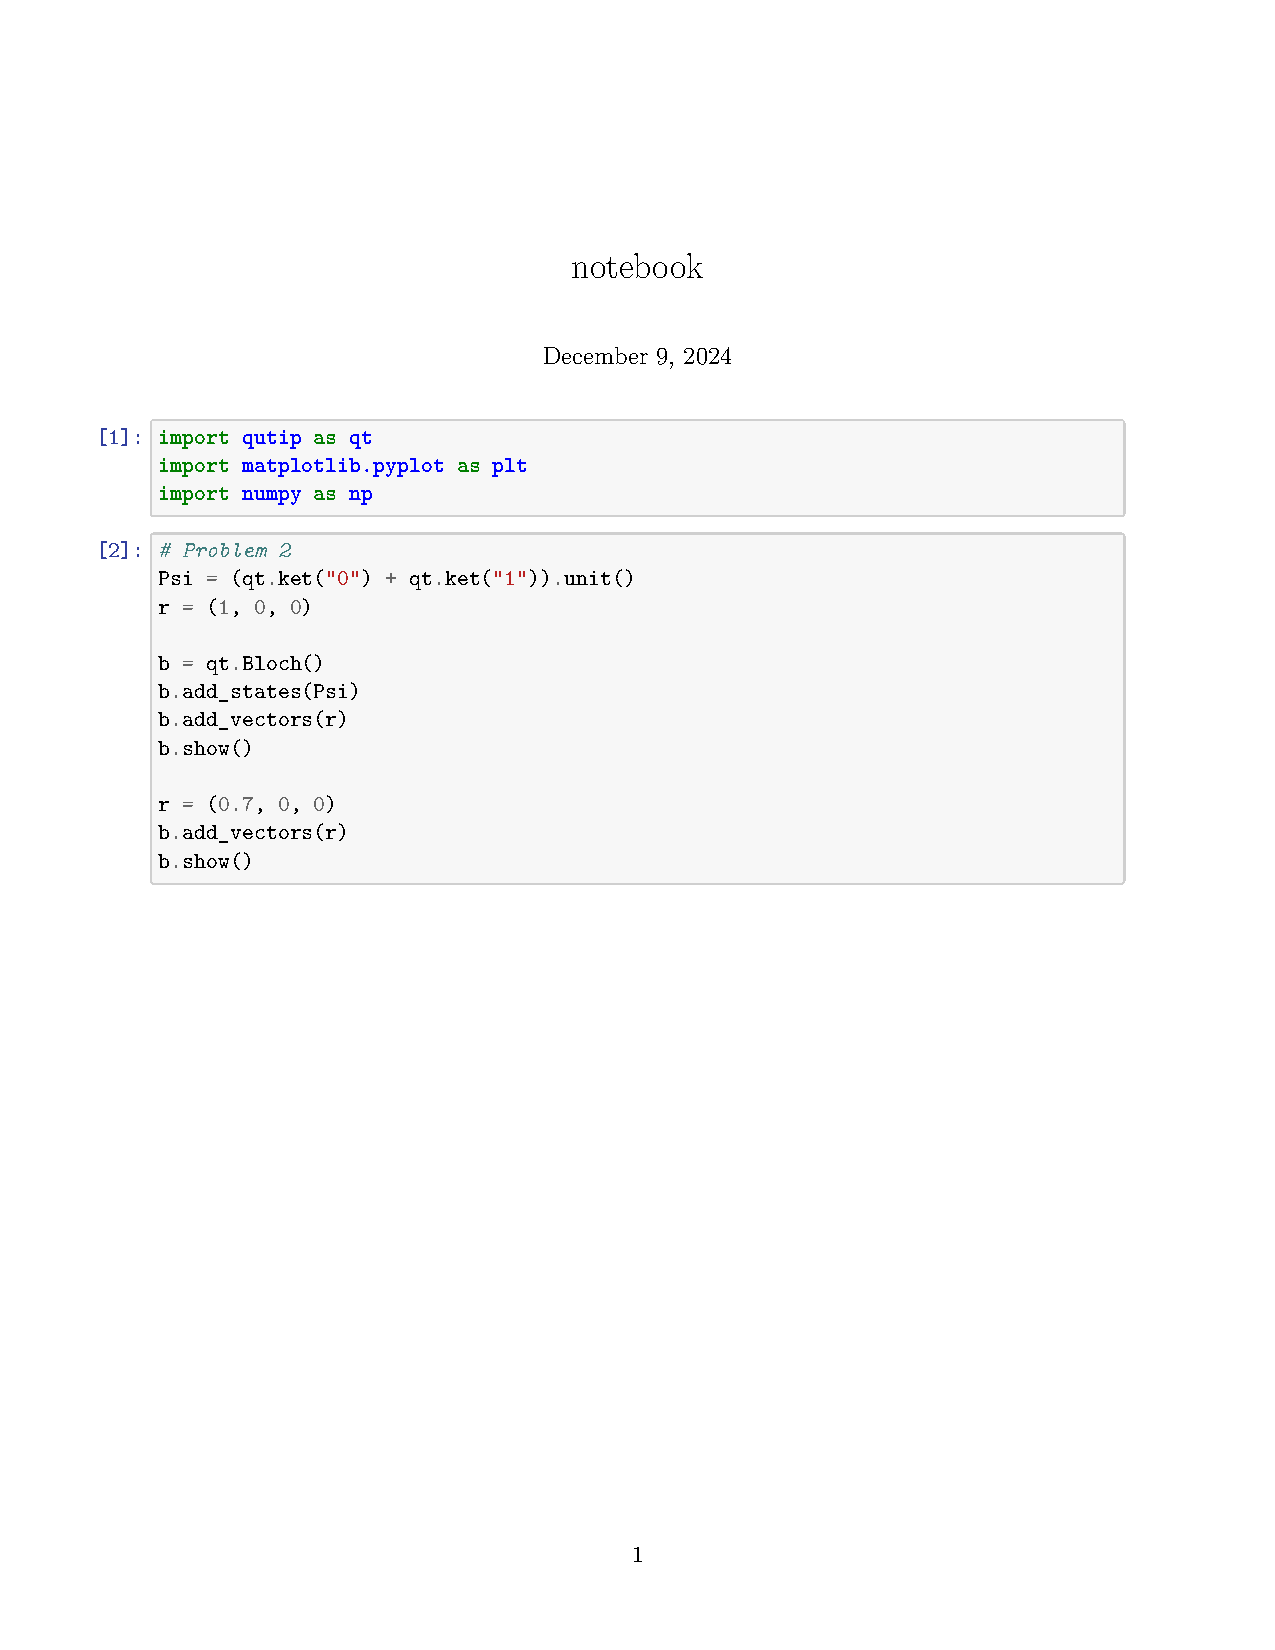
\includepdf[pages=-]{notebook.pdf}
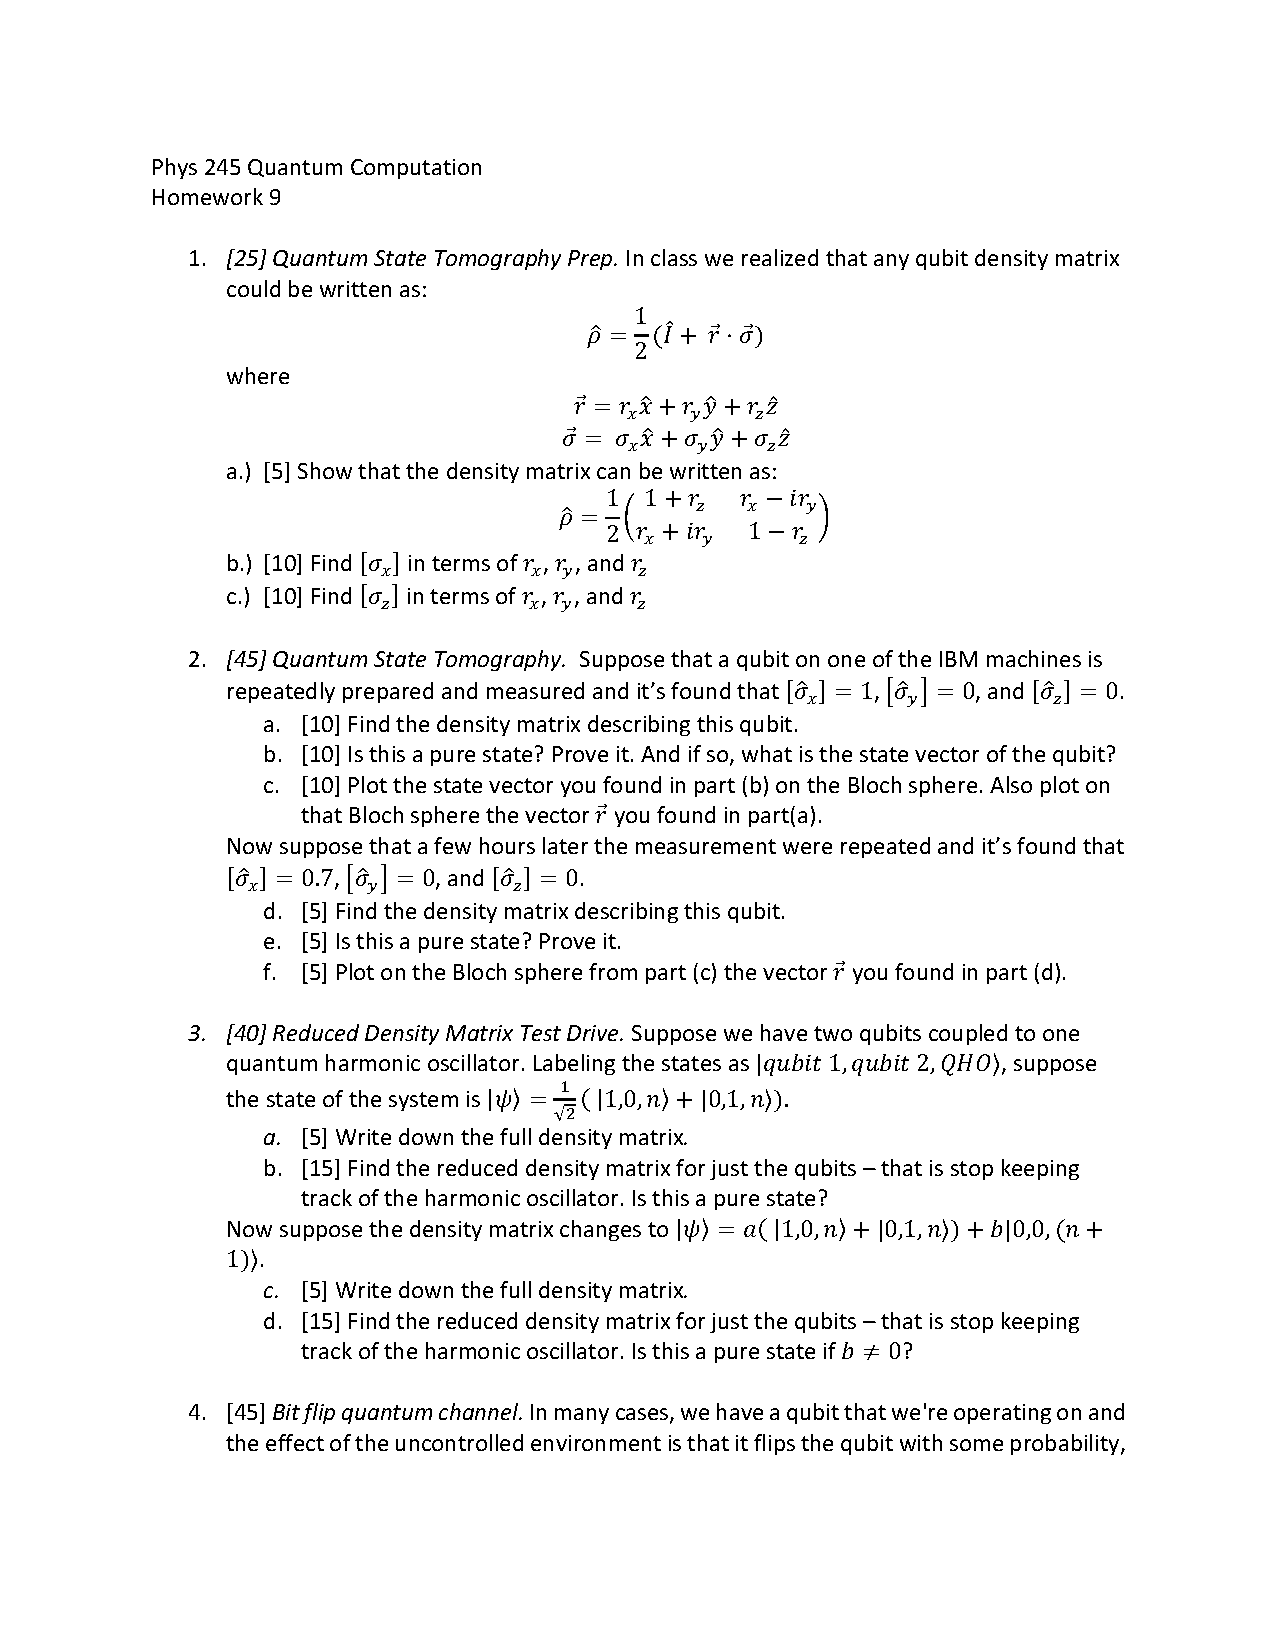
\includepdf[pages=-]{assignment.pdf}

\end{document}
